\documentclass{article}[A4]

% packages used
\usepackage[english]{babel}
\usepackage[utf8]{inputenc}
\usepackage{hyperref}
\usepackage{amsmath}
\usepackage{natbib}
\usepackage{hyperref}
\usepackage{graphicx}

\hypersetup{
    colorlinks=false,
}
\urlstyle{same}

% meta information
\title{Detecting child unsafe videos using transcripts}
\author{Shritishma Reddy \& Pratik Kamble}
\date{April, 16th 2019}

\begin{document}
\maketitle

\section{Abstract}

In this project, we propose an end-to-end pipeline for the detection of child unsafe videos
using video transcripts. Given the spread of digital media and increase in media consumption
by kids (ages 3-12) over the past decade, there is a great need for the filtering of unsafe
content found within reach of said age group. While traditional parental systems do exist,
this would be an online scalable system, that would  only benefit from the increasing video
consumption.

\section{Introduction}

This pipeline has three phases:
\begin{itemize}
    \item{Data acquisition: Collection of a holistic video-transcript dataset representative
    of children viewing habits and trends.}
    \item{Unsafe pattern detection: Analyze speech patterns and clustering hotspot zones to
    form a timeline representation.}
    \item{Video Classification: Classification of videos into unsafe types,
    if unsafe, viz. religious, abusive, drug use, etc.}
\end{itemize}

\subsection{Data Acquisition}

The data acquisition process depends a lot on the type of genre distribution.
A study \citep{childtime} has found that  children consume just over three hours of media,
as of 2015; the numbers having since then gone up further. \\

The time spent with on screen media dramatically increases from the toddler to preschool to
school-age years. Children under two have a screen time average of 53 minutes per day.
This increases to almost two and a half hours per day among two to four year old and almost
three hours for kids in the five to eight year old range. By age eight, 96\% of children have
watched TV, 90\% have used a computer, 81\% have played console video games, and 60\% have
played games or used apps on a portable device. Thus by order of data-source, we should have
a dataset representative mainly of TV show content, followed by YouTube and lastly, game video data. \\

Luckily, all video footage from various sources can be obtained from YouTube, along with transcript
data. TV show snippets, actual online vlog and other consumable media, as well as video game footage
can be found on the streaming platform. \\

\subsection{Unsafe Pattern Detection}

Once we have the annotated data, we have to run through it and classify according to unsafe-ness. Once
criterion that is of importance is categories that may influence minds may be quite different from ones
for adolescents or adults.

\begin{figure}[!htb]
    \centering
    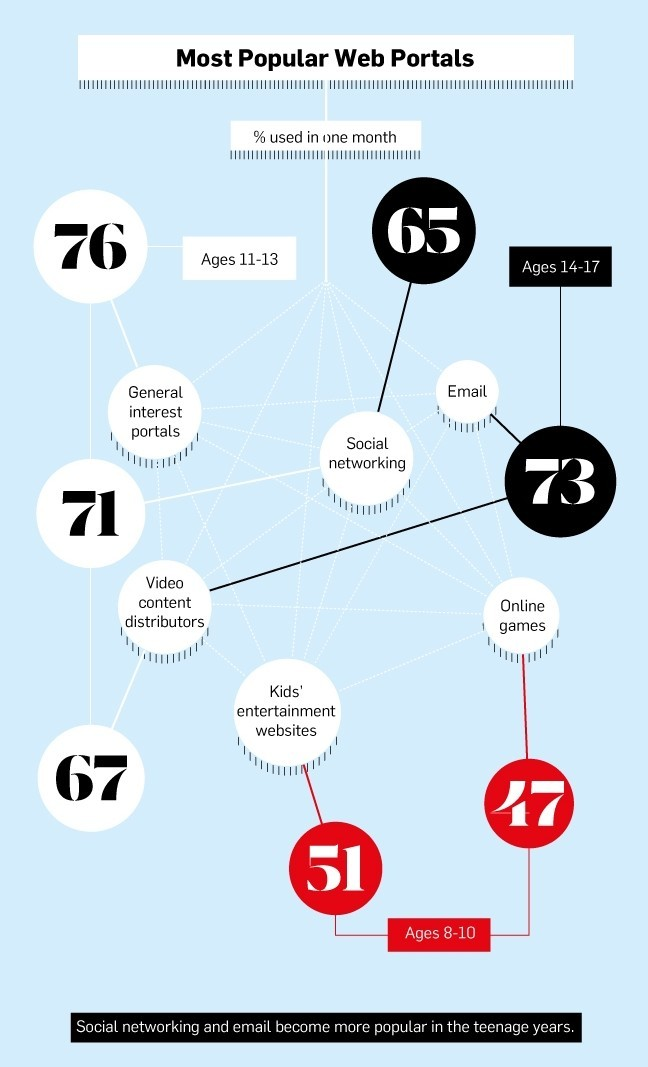
\includegraphics[scale=0.25]{graphic_stats.jpg}
    \caption{Major content sources and distribution}
    \label{fig:genre_dist}
\end{figure}

As seen from the figure \href{fig:genre_dist}, the main categories of media streaming are entertainment
websites, omline games, email, social networking and general interest portals. Breaking down the type of content
found on these sites, the main type of genres are as follows: \\
\begin{itemize}
    \item{Religion-based hate speech: This occurs in chatrooms and online forums, both high target kid influence}
    \item{Color-based hate speech: Depending on race and ethnicity, such sort of speech may be hidden in meaning and
    harder to detect.}
    \item{Foul Language: Kids usually pick up on foul language and the age of such exposure is lower this decade
    than it ever was.}
    \item{Other offensive terminology: Dealing with kids in the lower age bracket, systems need not worry too much about false positives,
    because of the ease of influence of media on early youth.}
\end{itemize}

\subsection{Video Classification}

Once the data collection for the transcripts is done, a simple classical model is used in cascade, to first analyze
and mark scenes and zones in the time frame with dangerous content.\\

This meta information is then passed to a zonal mapping pipeline, that, depending on how many zones of what clusters there are,
estimates a score for each category mentioned prior. Finally, depending on the thresholding for each genre distribution across ages,
a weighted average will judge the videos overall scores.

% Annotation process and ground truth collection
\section{Annotation and labeling}

The first step in the pipeline is the data collection and annotation. It is important to keep in mind the divisons
and genre distribution amidst children and have a dataset representative of that. We are collecting 5 videos in each positive category,
approximately of 5 minutes each, unless the genre specifies (eg, vlogs are usually longer). The videos should be at such an age genre balance
that younger children usually are pressured into by peers, and boundary videos are easy gateways to explicit content. \\

This gives us a total of 4 categories of positive videos, for each age group bracket within kids, targetting most common videos in the given set.

$$
N = n_{videos} \times n_{categories} \times n_{age groups} \times m \times \delta \times \alpha
$$

Here $n_{videos}$ is 5 per category, $n_{age groups}$ is 3, $m$ being the average length per video of selection. Now the average rate of speech
is $\delta$. This may vary across various demographics, but we choose the global average, 110 words per minute. Let's assume, since we are targetting
positive samples to seed the dataset, there is a 20\% conversion rate, $\alpha$. This means that 1 minute in a positive truth, 5 minute video contains
positive samples of the content we're trying to flag. This is a fair assumption, and goes in line with average statistics \citep{videostats}.

\subsection{Raw Transcript Collection}

After aggregating the various sources of media and content, our dataset consisted of 60 video subtitle files (*.srt). These files were formatted using the srt standard and had to be converted into a `DataFrame` for annotation. After cleaning invalid records and repeat rows, we were left with around 7000 observations.

\subsection{SRT Parsing and Dataset Aggregation}

Once we had a collection of formatted transcripts, they had to be aggregated and labeled. Each record of the dataset is of the form:
\begin{verbatim}
 Vedio_Id	Genre       start     end       text 
0  3tgZ...      0       0.00   3.71  mr. mine you say babe ...
1  3tgZ...      0       3.72  22.79  mr. mine babe what's d...
2  3tgZ...      0      22.79  22.80  of a dynamic punch mr. line 
3  3tgZ...      0      22.80  28.40  of a dynamic punch you'll... 
4  3tgZ...      0      28.40  28.41  you'll get stronger your 
\end{verbatim}

Every sample has a start and end marker, the genre for the video, and other meta information (as seen above). The timestamps and genre will help correlate the overall accuracy of the system with certain trends and patterns across genres. Additionally, some inference can be drawn as to the average "unsafe" duration of a video and the subsequent variation with genres. \\

Now, this annotated data is passed onto the model. The preliminary embedding and tagging of every sentence of a video is handled by the same. The results from said model are then passed onto an aggregator; it takes into account sentence based transcript data, augments it with additional meta information about the video and then makes a prediction regarding the safety of the video in terms of child consumption.

% Tagging of every sentence
\section{Model - Sentence labeling}

The model choice we ultimately went with was a bi-LSTM model with a simple embedding layer (from Keras). We used sequence model architectures i.e., BLSTM with character grams as inputs for training. BLSTM and LSTM models usually consists of three sequential layers:
\begin{itemize}
	\item{Embedding Layer}
	\item{Bidirectional LSTM}
	\item{Fully Connected Layer}
\end{itemize}

To compare the benefits of this model against other classical/hybrid approaches, we trained a model using classical approaches.\citep{hateoffensive}. Across the board, the accuracy of the chosen model was better than all other models considered (\textit{a comparitive analysis has been provided in the \textbf{results} section.}) A small improvement to the pipeline could be considered at this stage, viz. an ensemble approach with a mix of this bi-lstm model and a more classical approach.

\subsection{Structure}


\begin{itemize}
	\item{To deal with complex structured conversation data, we plan to use word level trigrams to represent each conversation.}
	\item{Sequence of trigrams sent through an embedding layer which takes one-hot vector of each character trigram in the sentence and learns the lower dimension representation for it.}
\end{itemize}

\subsection{Functionality \& Reasoning}

\begin{itemize}
	\item{Bi-Directional LSTMs have the ability to capture much richer sequential patterns from both directions of a sequence.}
	\item{Each character trigram from the previous embedding layer is fed as a sequence of trigrams, to the BLSTM layer.}
	\item{The output of the BLSTM layer is given as input to a Fully Connected (FC) layer which models the interactions between these features.}
	\item{The final softmax node in the FC layer outputs the probability of the sentence belonging to the inappropriate class.}
\end{itemize}



The initial training and validation was done on the Davidson dataset. This model gave excellent results, resulting in 99\% training accuracy and 89\% test accuracy on the baseline dataset. Results on the test dataset and comparison across all models is presented in the \textit{results} section.

% Overall video classification on basis of transcript clustering
\section{Zonal clustering and overall classification}

All the transcript data has been labeled as follows:
\begin{itemize}
\item {$\begin{bmatrix}1 & 0 & 0\end{bmatrix}$ Abusive}
\item {$\begin{bmatrix}0 & 1 & 0\end{bmatrix}$ Hate}
\item {$\begin{bmatrix}1 & 1 & 0\end{bmatrix}$ Abusive + Hate}
\item {$\begin{bmatrix}0 & 0 & 1\end{bmatrix}$ Clean}
\end{itemize}

This data is then mapped into a timeline heat map to indicate stronger zones of the video that may be unsafe. As part of the further work, this is the step wherein more meta information, age group, region, etc would be added so as to provide a better guess as part of the second phase (\textit{something like an additional FC layer, with the transcript heatmap as a feature subset}). \\

Now, as part of the first post processing step, we take the labeled video timeline and calculate the percentage of the video that's "unsafe". This is then cross-referenced with the genre based averages and an appropriate genre is determined. Once this part has been done, each genre has a statical threshold for it's unsafeness (again, precalculated). If the video then falls beyond such a threshold then, it is classified as unsafe. Additionally, it is run across other averages as well, and a score is given depending on the sensitivity of the system (\textit{higher sensitivity would lead to more false positives}). \\

These are then the final labels that are taken into account. As part of the results section, we have compared the end-to-end accuracy with ground truth obtained from manual viewing and judgment.

% Results at the end
\section{Results}

\subsection{Data preparation \& model training}
\subsubsection{Data preparation}
We have used Davidson dataset and 20\% of data corresponding to each label of our YouTube dataset for training. The Davidson dataset primarily consists of tweets. Hence, urls, hashtags, punctuation, user mentions etc are removed initially.
 All the sentences are then lemmatized and stemmed. Stopwords are also removed from all the sentences. Since, we are using a tfidf based tokeniser, removing stop words improves the rank of relevant words in the tokeniser. We use this clean data to train our tokeniser.
 From the above preprocessed dataset, we take all the words and train a glove model and get glove embeddings for the words in our training data. 
\subsubsection{Model Training}
\\*
\textbf{Classical Approach:}\\*
This model has been proposed by ?Automated Hate Speech Detection and the Problem of Offensive Language." ICWSM.
\\*
\textbf{Features} 

\begin{itemize}
	\item{We lowercased each sentence and stemmed it using the Porter stemmer, then create bigram, unigram, and trigram features, each weighted by its TF-IDF.}
	\item{To capture information about the syntactic structure we use NLTK (Bird, Loper, and Klein 2009) to construct Penn Part-of-Speech (POS) tag unigrams, bigrams, and trigrams}
	\item{To capture the quality of each tweet we use modified Flesch-Kincaid Grade Level and Flesch Reading Ease scores, where the number of sentences is fixed at one.}
	\item{We also use a sentiment lexicon designed for social media to assign sentiment scores to each tweet (Hutto and Gilbert 2014).}
	\item{We also include binary and count indicators for features for the number of characters, words, and syllables in each sentence.}
\end{itemize}
\\*
\textbf{Model} 
\begin{itemize}
\item{We first use a logistic regression with L1 regularization to reduce the dimensionality of the data.}
\item{We tested each model using 5-fold cross validation, holding out 10\% of the sample for evaluation to help prevent overfitting.}
\item{After using a grid-search to iterate over the models and parameters we find that the Logistic Regression and Linear SVM tended to perform significantly better than other models.}
\item{We decided to use a logistic regression with L2 regularization for the final model.}
\item{We trained the final model using the Davidson dataset and used it to predict the label for each sentence of Youtube Transcript Dataset.}
\item{We use a one-versus-rest framework where a separate classifier is trained for each class and the class label with the highest predicted probability across all classifiers is assigned to each tweet.}
\item{All modeling was performing using scikit-learn.}
\end{itemize}
\begin{figure}[!htb]
    \centering
    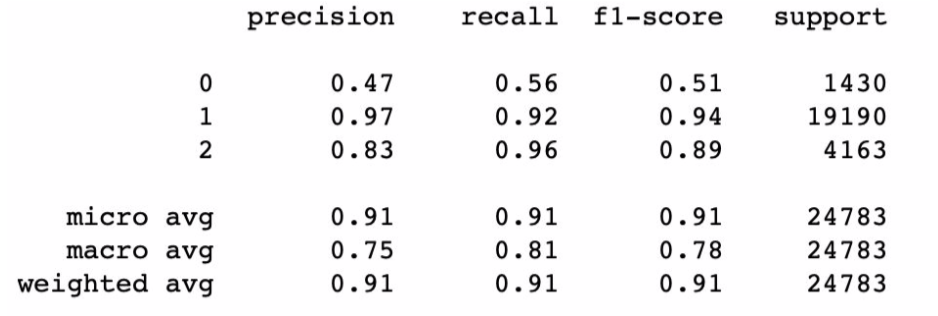
\includegraphics[scale=0.50]{classical.png}
    \caption{Classical training}
    \label{fig:model_res}
\end{figure}
\\*
\textbf{Bi-LSTM Model:}\\*
\textbf{Model} 
\begin{itemize}
\item{We use an initial Embedding Layer to which we give our trained glove embeddings as weights. }
\item{Bi-Directional LSTMs have the ability to capture much richer sequential patterns from both directions of a sequence.}
\item{The output of the BiLSTM layer is given as input to a Fully Connected (FC) layer which models the interactions between these features.}
\item{Then 2 Dense layers with appropriate drop out ratios are added sequentially.}
\item{The final soft-max node in the FC layer outputs the probability of the sentence belonging to the inappropriate class}
\end{itemize}
\begin{figure}[!htb]
    \centering
    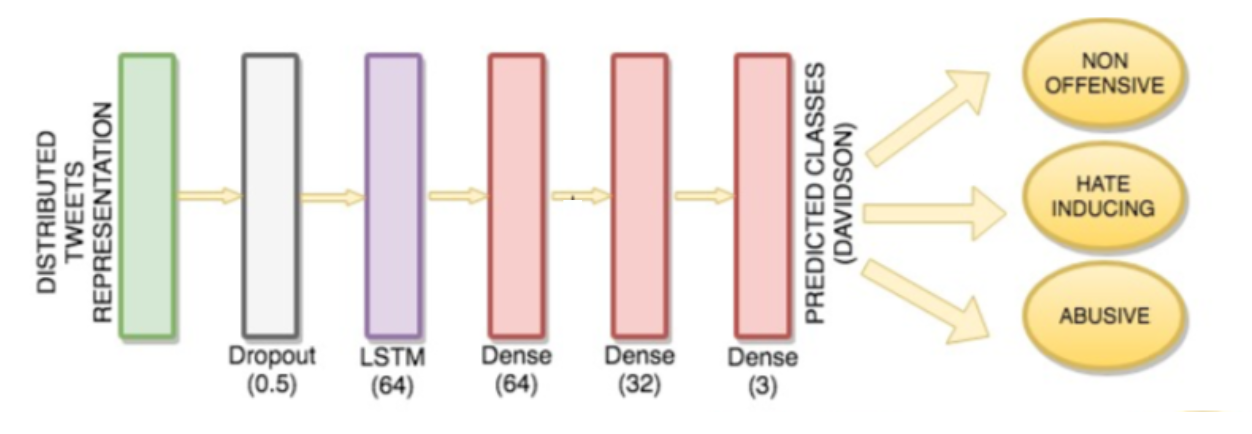
\includegraphics[scale=0.50]{model.png}
    \caption{Architecture}
    \label{fig:model_res}
\end{figure}

\subsection{Final Choice \& Testing}

\subsection{Pipeline results}

% Success rate and scalable component
\section{Conclusion \& further work}

Given the two step process of "classification", some interesting results can be drawn. From the dataset that we collected, we noticed:
% TODO: add information here about the final classifications and other interesting patterns

\subsection{Further Work}

Thus, with the classification methods of the bi-lstm model with a combination of the classical method should give us the best performance. Additionally, information from the classical method can be used in the later clustering and analysis step. A later step is to provide a finer analysis of the type of content and possibly give an appropriate age rating, though this might require some additional work. \\

Another improvement on the to-do list is to supplement the timeline information with more features, say region and appropriate age group. This way, an online learning model would be able to learn trends in consumption behaviour and auto-adjust to regional trends and filtering.

You can find the complete codebase, along with some helpful scripts on \href{https://github.com/Pk13055/transcript-based-classification}{GitHub}. Feel free to contribute and request features!

\bibliographystyle{plain}
\bibliography{references}
\end{document}
